\documentclass{beamer}

\usepackage{graphicx}
\usepackage{caption}

\mode<presentation>
{
  \usetheme{Darmstadt}

  \setbeamercovered{transparent}
}

\DeclareMathOperator*{\argmax}{arg\,max}
\DeclareMathOperator*{\argmin}{arg\,min}

\title{Gradient Coding}

\author{Runtian Zhu \\ \texttt{zhurt23@m.fudan.edu.cn}}

\date{2023.11.9}

\begin{document}

\captionsetup[figure]{labelformat=empty}

\begin{frame}
  \titlepage
\end{frame}

\section{Reference}

\begin{frame}{Reference}

\begin{itemize}
    \item R. Tandon, Q. Lei, A. G. Dimakis, and N. Karampatziakis, “\textbf{Gradient coding: Avoiding stragglers in distributed learning},” in International Conference on Machine Learning, PMLR, 2017, pp. 3368–3376.
\end{itemize}

\begin{figure}
    \centering
    \begin{minipage}[t]{.2\paperwidth}
        \centering
        
\includegraphics[width=\textwidth]{res/Rashish Tandon.jpg}
        \caption{Rashish Tandon}
    \end{minipage}
    \begin{minipage}[t]{.2\paperwidth}
        \centering
        
\includegraphics[width=\textwidth]{res/Qi Lei.jpg}
        \caption{Qi Lei}
    \end{minipage}
    \begin{minipage}[t]{.2\paperwidth}
        \centering
        
\includegraphics[width=\textwidth]{res/alexdimakis_sm.jpg}
        \caption{Alexandros G. Dimakis}
    \end{minipage}
    \begin{minipage}[t]{.2\paperwidth}
        \centering
        
\includegraphics[width=\textwidth]{res/Nikos Karampatziakis.jpg}
        \caption{Nikos Karampatziakis}
    \end{minipage}
\end{figure}

\end{frame}

\section{Background}

\begin{frame}
    \frametitle{Machine Learning: Regression}

    \begin{block}{Regression}
        Given a data set $D = \{(\boldsymbol{x}_1, \boldsymbol{y}_1), \dots, (\boldsymbol{x}_N, \boldsymbol{y}_N)\}$. The goal is to find a function $f_{\hat{\boldsymbol{\theta}}}$ from some function space $F = \{f_{\boldsymbol{\theta}} \vert \boldsymbol{\theta} \in \mathbb{R}^m\}$ such that
        \[\hat{\boldsymbol{\theta}} = \argmin_{\boldsymbol{\theta}} L(\boldsymbol{\theta})\]
    \end{block}
    
    \begin{block}{Loss Function: Mean Squared Error (MSE)}
        \[L(\boldsymbol{\theta}) = \frac{1}{N}\sum_{i = 1}^{N} \lVert\boldsymbol{y}_i - f_{\boldsymbol{\theta}}(\boldsymbol{x}_i)\rVert^2\]
    \end{block}

    \[D = \{(0, 0), (1, 1), (-1, 0)\},\; F = \{x^2 + ax + b \vert a, b \in \mathbb{R}\}, \;\boldsymbol{\theta} = \begin{bmatrix}
        a \\
        b
    \end{bmatrix}\]

\end{frame}

\begin{frame}{Gradient Descent in Machine Learning}

\begin{block}{Gradient Descent}
    \[\boldsymbol{\theta}_{k + 1} = \boldsymbol{\theta}_{k} - \alpha\boldsymbol{\nabla} L(\boldsymbol{\theta}_{k})\]
\end{block}
    
\begin{block}{Loss Function: Mean Squared Error (MSE)}
    \[L(\boldsymbol{\theta}) = \frac{1}{N}\sum_{i = 1}^{N} \lVert\boldsymbol{y}_i - f_{\boldsymbol{\theta}}(\boldsymbol{x}_i)\rVert^2\]
    \[\boldsymbol{\nabla}L(\boldsymbol{\theta}) = \sum_{i = 1}^{N}\frac{\partial\frac{1}{N}\lVert\boldsymbol{y}_i - f_{\boldsymbol{\theta}}(\boldsymbol{x}_i)\rVert^2}{\partial\boldsymbol{\theta}}\]
\end{block}

\end{frame}

\begin{frame}{Distributed Learning}{Straggler Problem}
    \begin{columns}
        \begin{column}{0.6\textwidth}
            \begin{block}{Problem Setting}
                Given data sets $D_1, \dots, D_k$ ($D_i$ can be viewed as a vector). Each round, a parameter $\boldsymbol{\theta}$ is given. Calculate $\boldsymbol{g}_{\boldsymbol{\theta}}(D_1) + \dots + \boldsymbol{g}_{\boldsymbol{\theta}}(D_k)$.
            \end{block}
            Problem:
            \begin{itemize}
                \item Some workers may be stragglers (work much slower)
            \end{itemize}
            
        \end{column}
        \begin{column}{0.48\textwidth}
            \begin{figure}
                \centering
                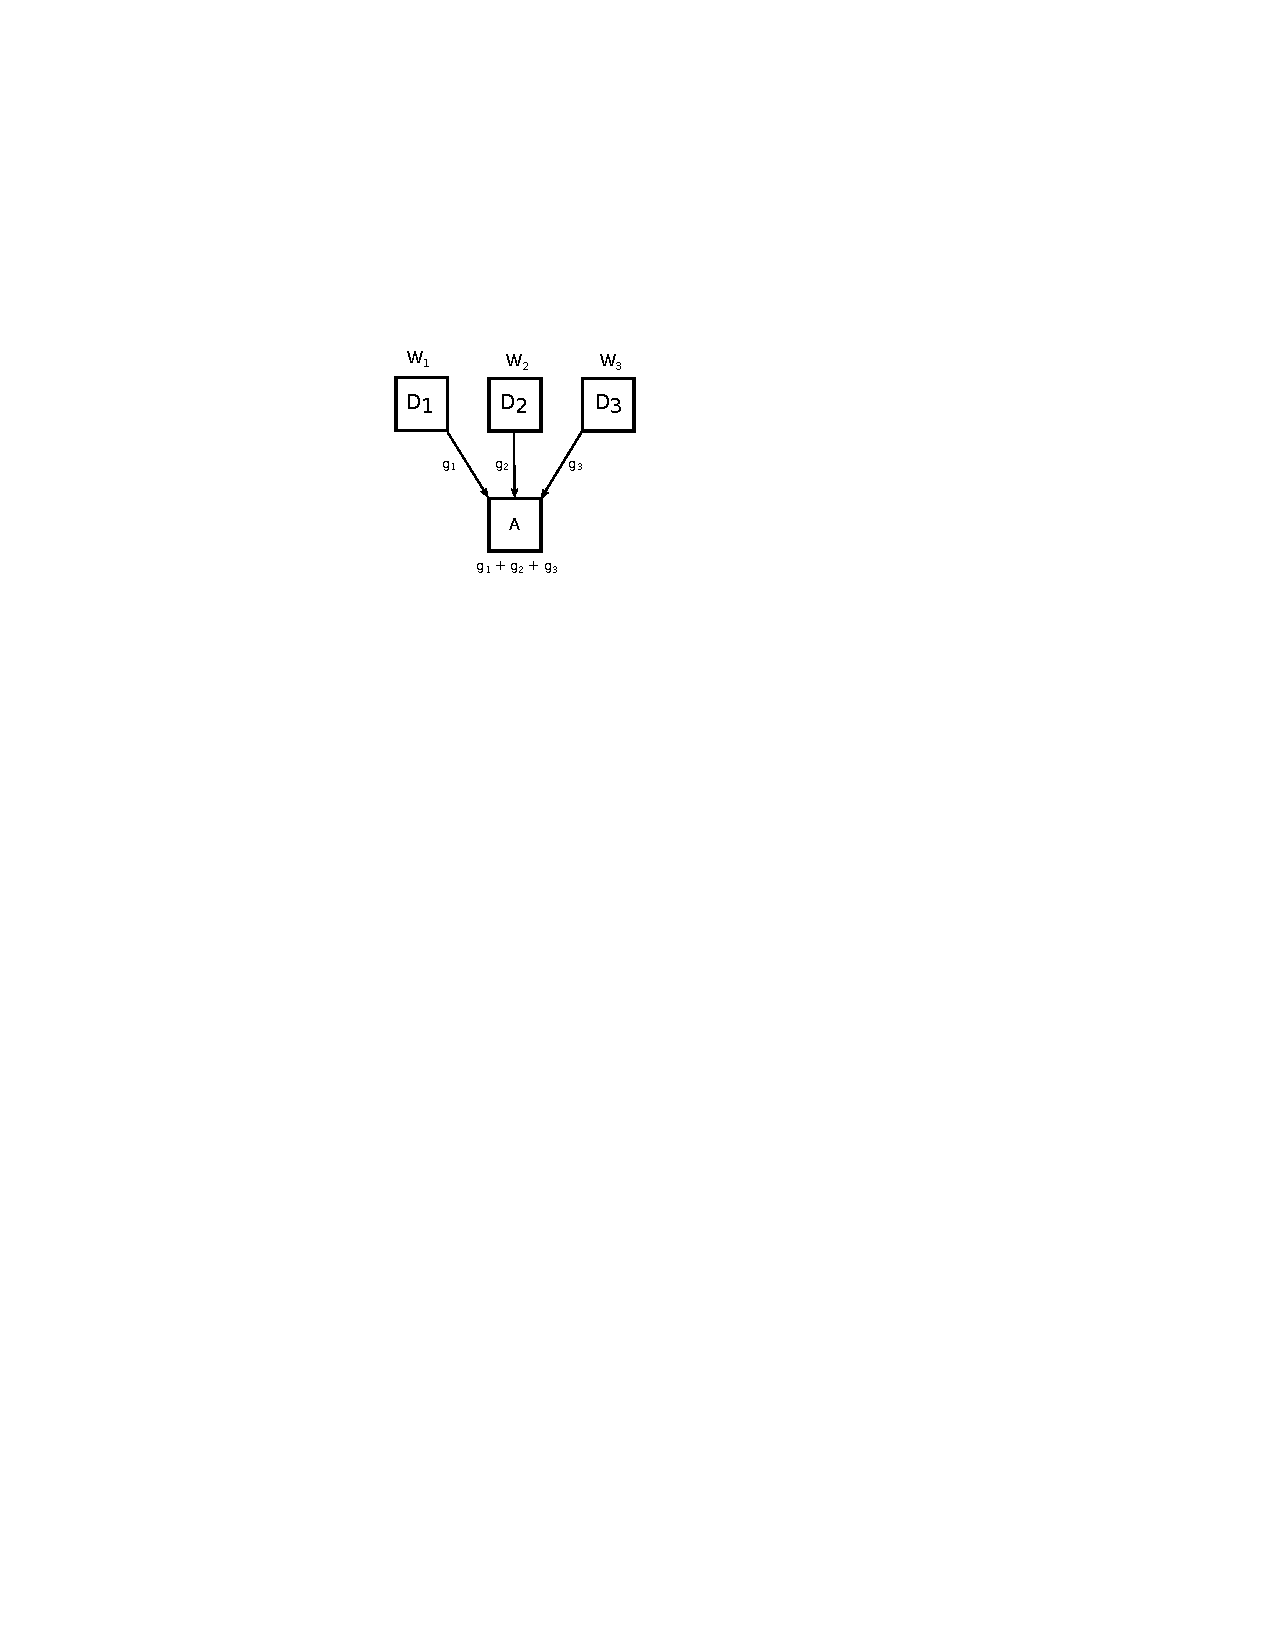
\includegraphics[height=.5\textheight]{res/distributed_learning.pdf}
            \end{figure}
        \end{column}
    \end{columns}
\end{frame}

\begin{frame}{Distributed Learning}{Solution: replication}

\begin{figure}
    \centering
    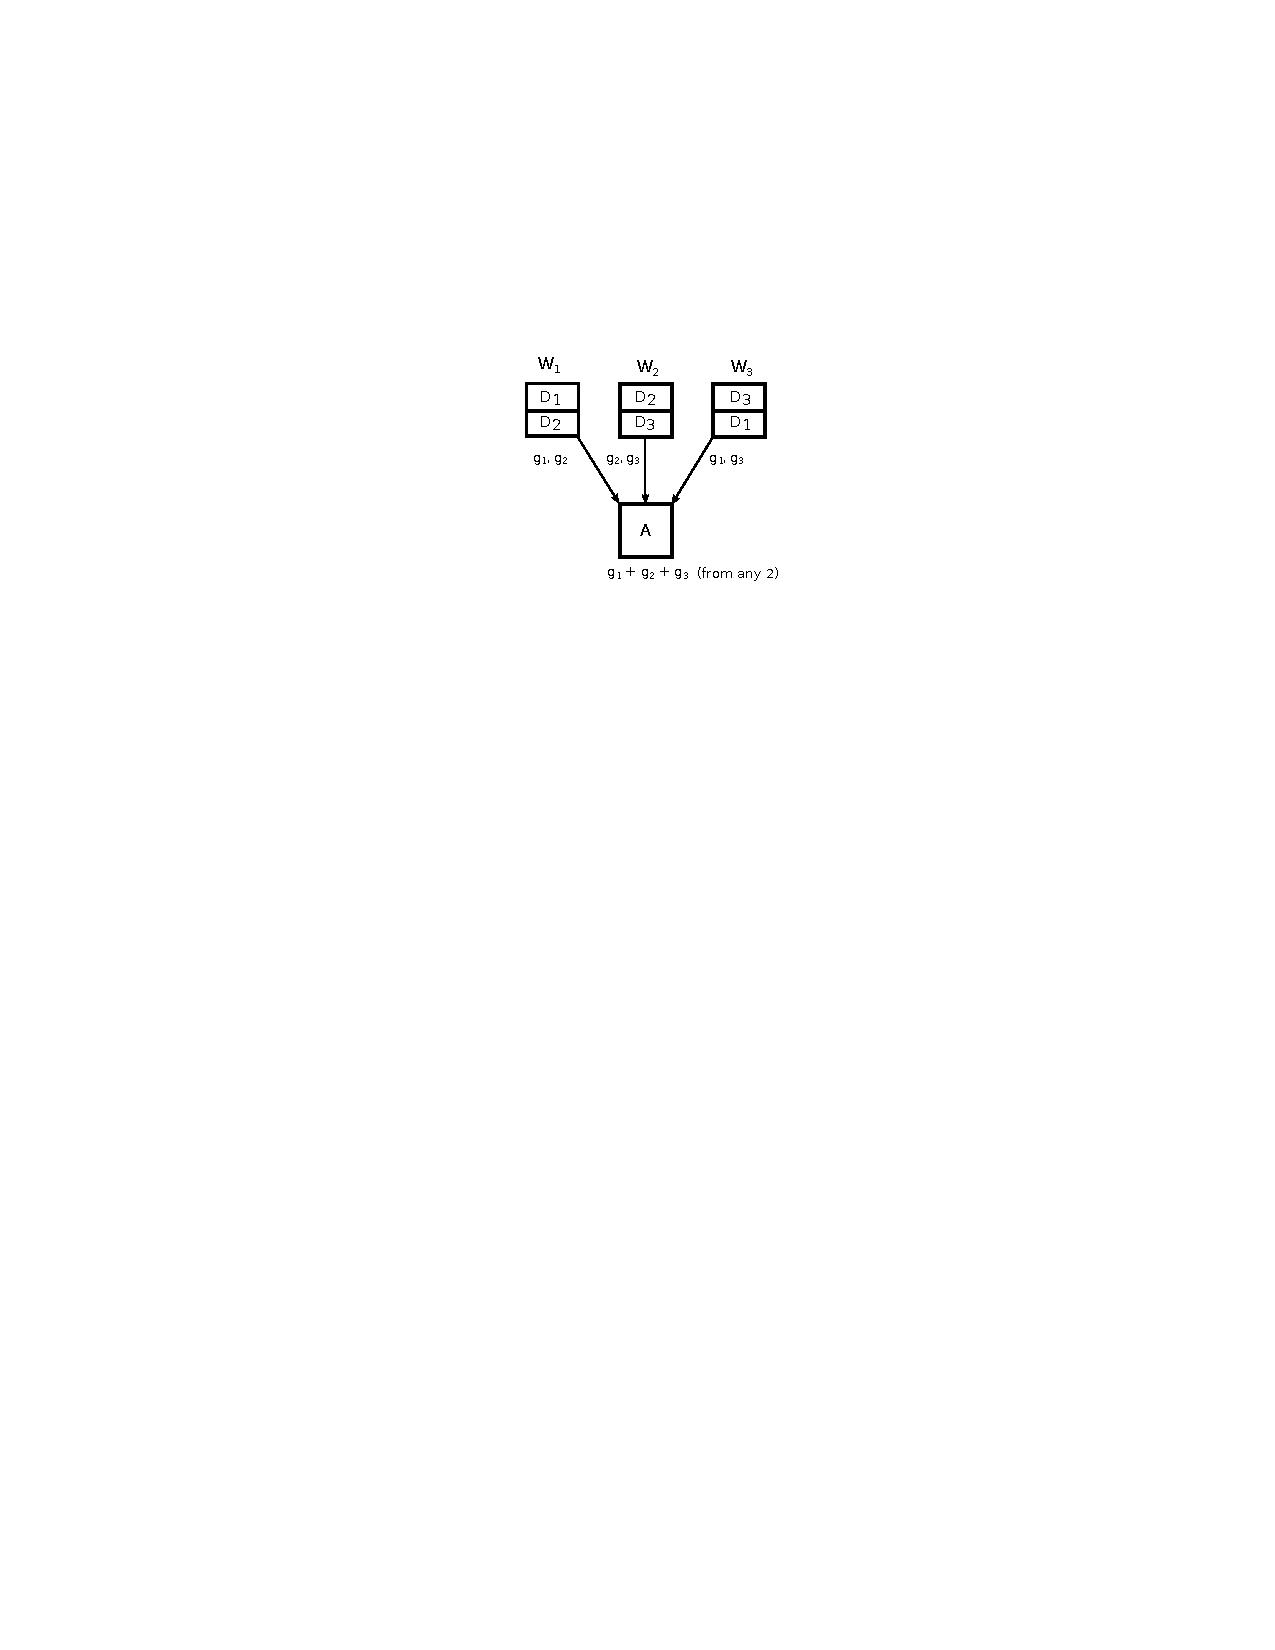
\includegraphics[height=.7\textheight]{res/replicate.pdf}
\end{figure}

\end{frame}

\begin{frame}{Distributed Learning}{Gradient Coding}

\begin{figure}
    \centering
    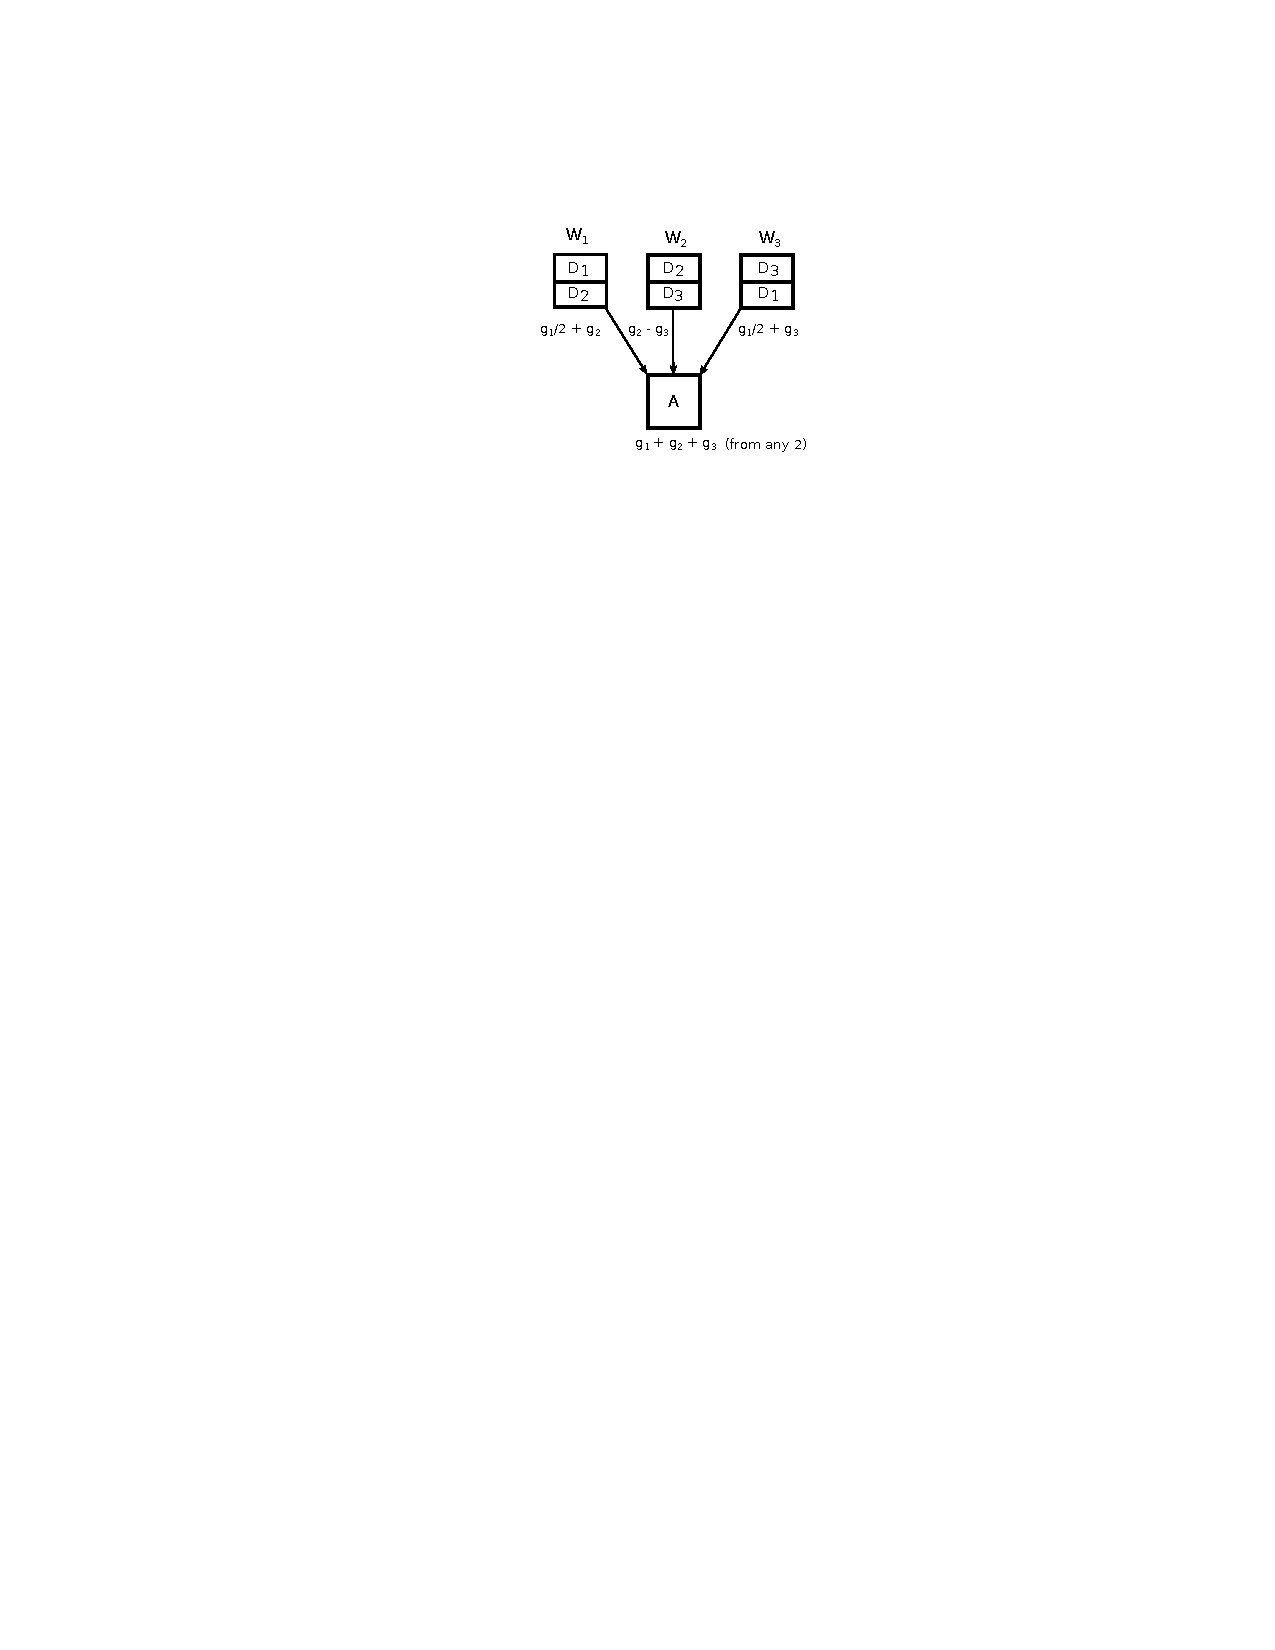
\includegraphics[height=.7\textheight]{res/gradient coding.pdf}
\end{figure}

\end{frame}

\section{Gradient Coding}

\subsection{General Case}

\begin{frame}{Gradient Coding}{The General Setup}

\begin{definition}
    Let $f$ denotes the number of combinations of surviving workers/non-stragglers, $n$ denotes the number of workers, $k$ denotes the number of data partitions.
\end{definition}

\begin{definition}
    Let $A \in \mathbb{R}^{f \times n}$, the $i^{th}$ row of $A$ be $\boldsymbol{a}_i$. Each row of $A$ indicates a combination of surviving workers/non-stragglers.
\end{definition}

\begin{definition}
    Let $B \in \mathbb{R}^{n \times k}$, the $i^{th}$ row of $B$ be $\boldsymbol{b}_i$. $\boldsymbol{b}_i$ indicates the data partitions that the $i^{th}$ worker has access to.
\end{definition}

\end{frame}

\begin{frame}{Gradient Coding}{The General Setup}

\begin{block}{Conditions to be Met}
    \[AB = \boldsymbol{1}_{f\times k}\]
\end{block}

\begin{columns}

\begin{column}{.5\linewidth}
        
\begin{Example}
    \[A = \begin{bmatrix}
        0 & 1 & 2 \\
        1 & 0 & 1 \\
        2 & -1 & 0
    \end{bmatrix}\]
    
    \[B = \begin{bmatrix}
        1/2 & 1 & 0 \\
        0 & 1 & -1 \\
        1/2 & 0 & 1
    \end{bmatrix}\]
\end{Example}
    
\end{column}

\begin{column}{.5\linewidth}

\begin{figure}
    \centering
    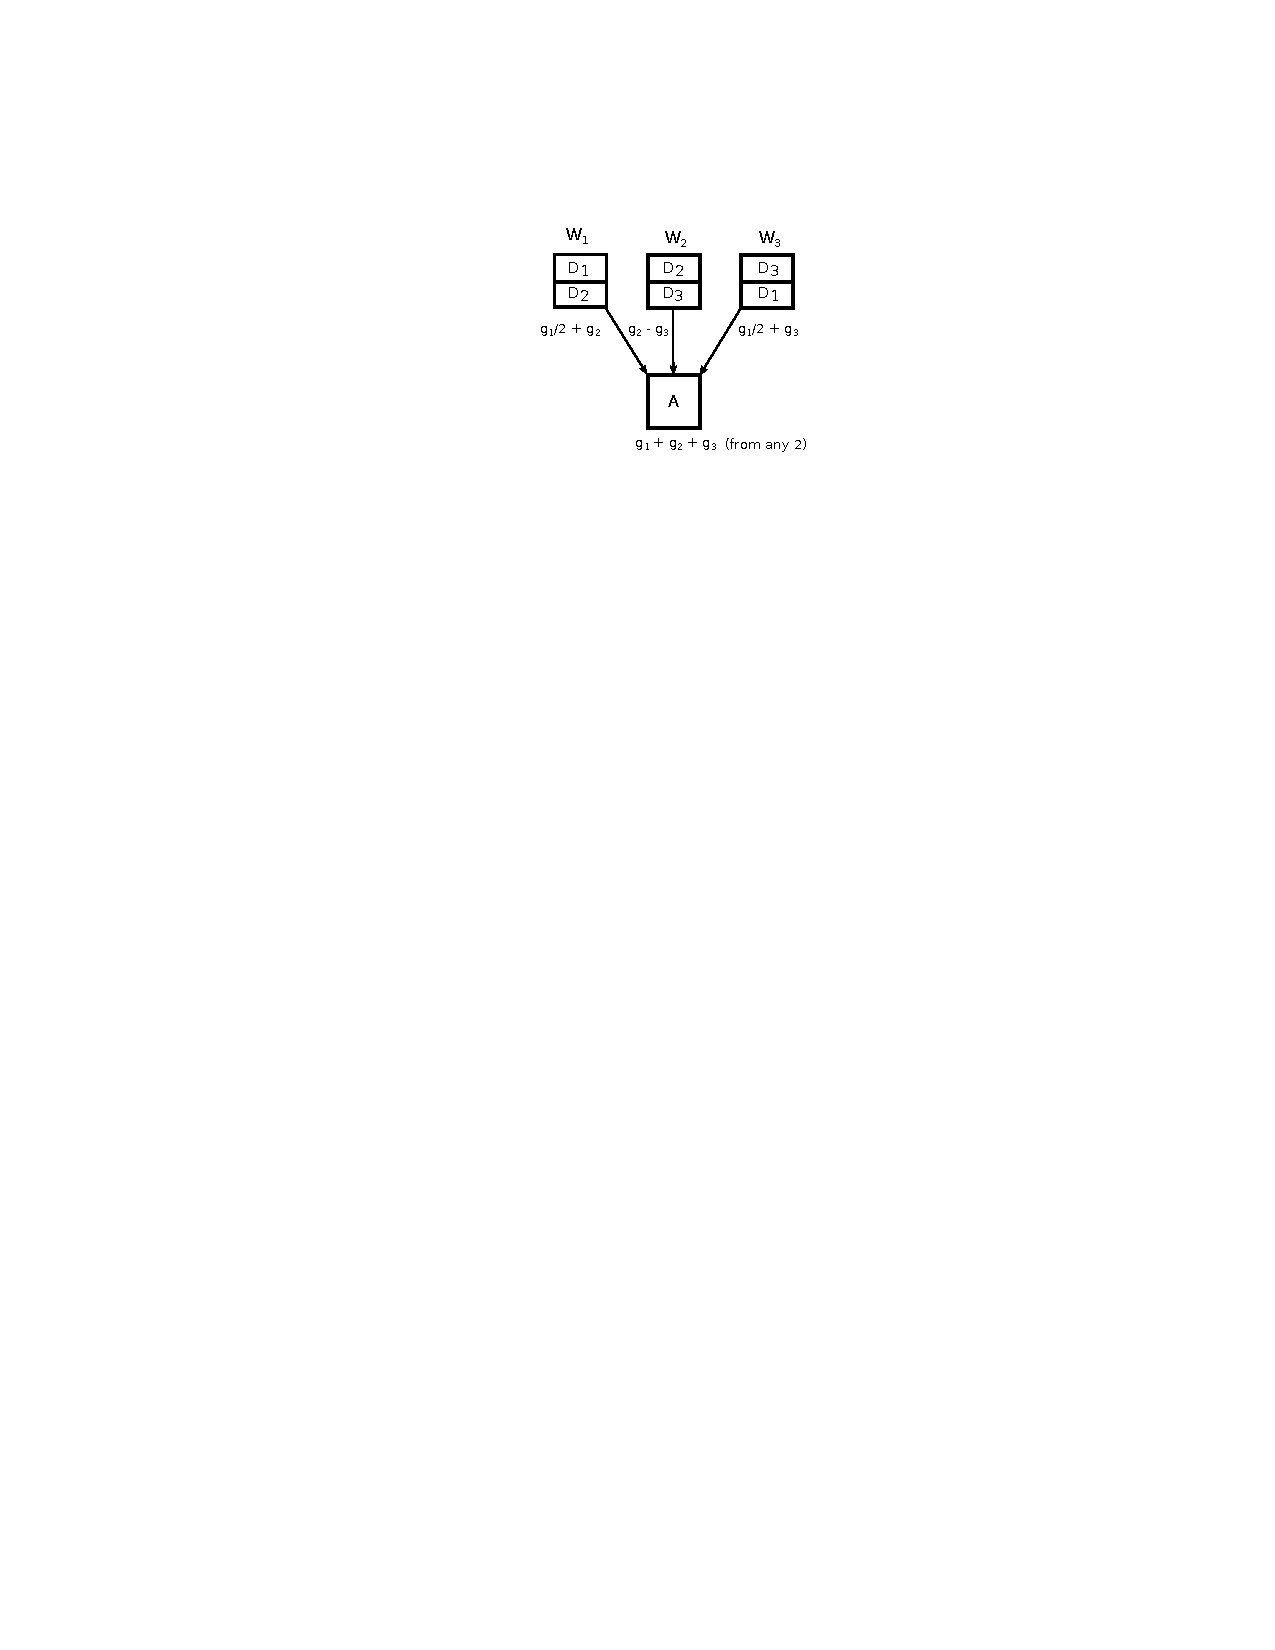
\includegraphics[width=\textwidth]{res/gradient coding.pdf}
\end{figure}

\end{column}

\end{columns}

\end{frame}

\begin{frame}{Gradient Coding}{The General Setup}

\begin{block}{Property}
    \[\boldsymbol{a_i}B\boldsymbol{\bar{g}} = \begin{bmatrix}
        1 & 1 & \dots & 1
    \end{bmatrix}\boldsymbol{\bar{g}} = (\sum_{j=1}^{k}\boldsymbol{g_j})^T\]
    \[\boldsymbol{a_i}B\boldsymbol{\bar{g}} = \sum_{k\in supp(\boldsymbol{a_i})}\boldsymbol{a_i}(j)(\boldsymbol{b_j} \boldsymbol{\bar{g}})\]
    where $\boldsymbol{\bar{g}} = \begin{bmatrix}
        \boldsymbol{g_1} & \boldsymbol{g_2} & \dots & \boldsymbol{g_k}
    \end{bmatrix}^T$, $\boldsymbol{g_i}$ denotes the gradient of the $i^{th}$ partition of work, $supp(\boldsymbol{x}) = \{i | x_i \neq 0\}$.
\end{block}


\end{frame}

\section{Further Work}

\subsection{DRACO}

\begin{frame}{DRACO}

    \begin{itemize}
        \item L. Chen, H. Wang, Z. Charles, and D. Papailiopoulos, “\textbf{Draco: Byzantine-resilient distributed training via redundant gradients},” in International Conference on Machine Learning, PMLR, 2018, pp. 903–912.
    \end{itemize}

\end{frame}

\subsection{Interactive Gradient Coding}

\begin{frame}{Interactive Gradient Coding}

    \begin{itemize}
        \item C. Hofmeister, L. Maßny, E. Yaakobi, and R. Bitar, “\textbf{Trading Communication for Computation in Byzantine-Resilient Gradient Coding},” arXiv preprint arXiv:2303.13231, 2023.
    \end{itemize}

\end{frame}

\end{document}

